\titledquestion{基于转移的神经依存句法分析}[54]

在这一部分，你将实现一个基于神经网络的依存句法分析器，目标是最大化 UAS（Unlabeled Attachment Score，无标签依存附着分数）指标。\newline

在开始之前，请按照 README 中的说明安装该作业所需的所有依赖。我们将使用来自 \url{https://pytorch.org/get-started/locally/} 的 PyTorch 2.1.2，并将 \texttt{CUDA} 选项设为 \texttt{None}；同时使用 tqdm 包，它会在训练过程中显示进度条。PyTorch 官方网站提供了大量教程，对理解 PyTorch 的 Tensor 库和神经网络非常有帮助。\newline

依存句法分析器会分析句子的语法结构，建立\textit{head}（核心词）和修饰这些核心词的词之间的关系。依存句法分析器有多种类型，包括转移式分析器、基于图的分析器和基于特征的分析器。你的实现将是一个{\it 转移式}分析器，它会逐步增量构建语法分析结果。每一步都维护一个\textit{partial parse}（部分分析），其表示如下：
\begin{itemize}
\item 一个当前正在处理的词{\it stack}（栈）。
\item 一个尚未处理的词{\it buffer}（缓冲区）。
\item 一个由分析器预测出的{\it dependencies}（依存关系）列表。
\end{itemize}
初始时，栈中只包含 ROOT，依存关系列表为空，缓冲区按原句顺序包含所有词。每一步，分析器都会对当前部分分析应用一个{\it transition}（转移），直到缓冲区为空且栈大小为 1。可以应用的转移如下：
\begin{itemize}
\item \texttt{SHIFT}：从缓冲区中移除第一个词并压入栈顶。
\item \texttt{LEFT-ARC}：将栈中第二个（最近加入的第二个）元素标记为第一个元素的从属词，并从栈中移除这个第二个元素，将一条 \textit{first\_word} $\rightarrow$ \textit{second\_word} 的依存关系加入依存关系列表。
\item \texttt{RIGHT-ARC}：将栈中第一个（最近加入的）元素标记为第二个元素的从属词，并从栈中移除第一个元素，将一条 \textit{second\_word} $\rightarrow$ \textit{first\_word} 的依存关系加入依存关系列表。
\end{itemize}
每一步，分析器都会使用神经网络分类器在这三种转移中做出选择。

\begin{parts}
    
    \part[4] \textcolor{black}{按照解析句子 {\it ``I presented my findings at the NLP conference''} 所需的转移顺序逐步操作。该句子的依存树如下图所示。每一步都给出栈和缓冲区的配置，以及该步应用了什么转移，以及新增了什么依存关系（如果有）。前三步已作为示例给出。} \\ 

    %\begin{center}
    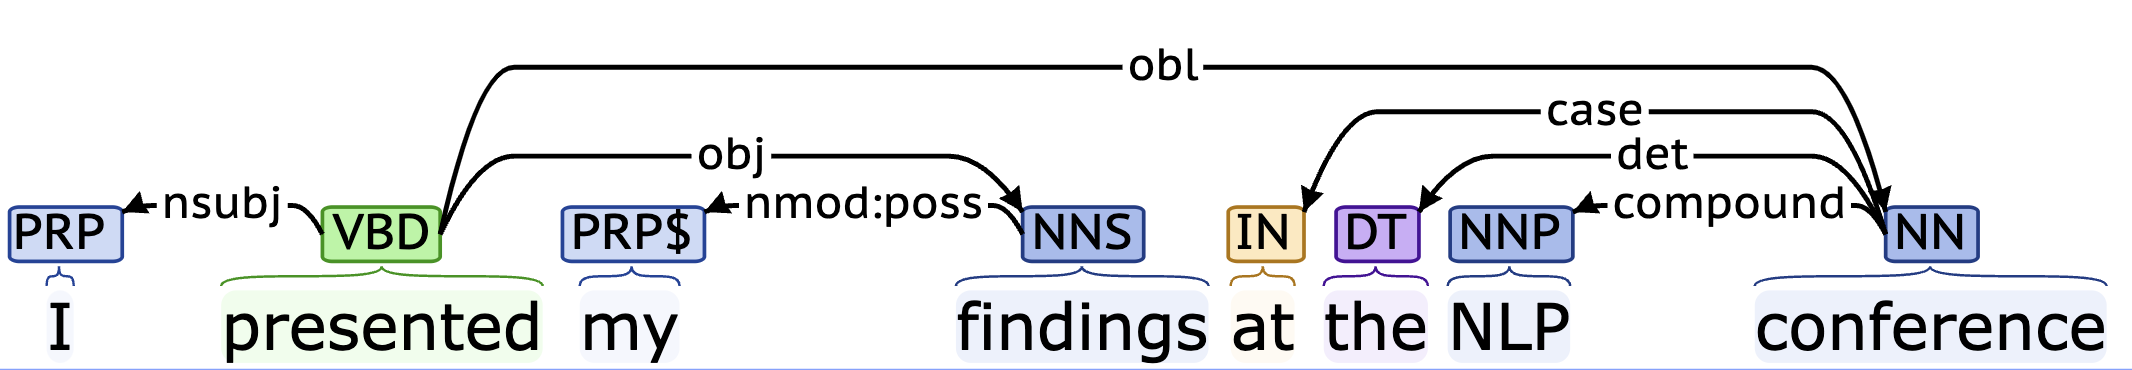
\includegraphics[width=0.8\textwidth]{example.png} \\
    %\end{center}

    \begin{adjustwidth}{-2cm}{}
    \begin{tabular}{ l | l | l | l}
    Stack & Buffer & New dependency & Transition \\ \hline
    [ROOT] & [I, presented, my, findings, at, the, NLP, conference] &  & Initial Configuration \\
    $[$ROOT, I] & [presented, my, findings, at, the, NLP, conference] &  &  \texttt{SHIFT}  \\
    $[$ROOT, I, presented] & [my, findings, at, the, NLP, conference] &  &  \texttt{SHIFT}  \\
    $[$ROOT, presented] & [my, findings, at, the, NLP, conference] & presented$\to$I &  \texttt{LEFT-ARC}  \\
    \end{tabular}\newline
    \end{adjustwidth}
    
    \part[2] 一个包含 $n$ 个词的句子需要多少步来完成解析（用 $n$ 表示）？请用 1--2 句话说明原因。

       
    
    \part[6] 在 \texttt{PartialParse} 类中实现 \texttt{\_\_init\_\_} 和 \texttt{parse\_step} 函数，位置在 \texttt{parser\_transitions.py}。它实现了分析器使用的转移机制。你可以运行 \texttt{python parser\_transitions.py part\_c} 来进行基础（非穷尽）测试。

    \part[8] 我们的网络将预测每个部分分析下一步应该应用哪个转移。我们可以用它逐个句子解析：持续应用模型预测的转移，直到解析完成；不过，神经网络在对\textit{批量}数据做预测时效率更高（即同时预测多个不同部分分析的下一步转移）。我们可以使用下面的算法对句子进行 minibatch 解析。\newline

    \alglanguage{pseudocode}
    \begin{algorithm*}[h]
    \caption{Minibatch Dependency Parsing}
    \begin{algorithmic}
    	\State \textbf{Input:} \texttt{sentences}，待解析句子的列表，以及 \texttt{model}，用于做解析决策的模型
    	%\State
    	%\State Initialize \texttt{partial\_parses} $\to$ []
    	%\For{\textbf{each} sentence \texttt{s} in \texttt{sentences}}
    	%\State Add a partial parse to \texttt{partial\_parses} with \texttt{stack} = [ROOT], \texttt{buffer} = \texttt{s}, \texttt{dependencies} = []
    	%\EndFor
    	\State
    	\State 将 \texttt{partial\_parses} 初始化为一组 PartialParses，每个句子对应一个
    	\State 将 \texttt{unfinished\_parses} 初始化为 \texttt{partial\_parses} 的浅拷贝
    	%\State
    	\While{\texttt{unfinished\_parses} 非空}

    	\State 取 \texttt{unfinished\_parses} 中前 \texttt{batch\_size} 个解析作为一个 minibatch
    	\State 用 \texttt{model} 对 minibatch 中每个部分分析预测下一步转移
    	\State 对 minibatch 中每个部分分析使用它预测到的转移执行一次解析步骤
    	\State 从 \texttt{unfinished\_parses} 中删除已完成的解析（缓冲区为空且栈大小为 1）
    	\EndWhile
    	\State
    	\State \textbf{Return:} \texttt{partial\_parses} 中每个（现已完成）解析的 \texttt{dependencies}。
    \end{algorithmic}
    \end{algorithm*}
    
    在 \texttt{parser\_transitions.py} 中实现 \texttt{minibatch\_parse} 函数。你可以运行 \texttt{python parser\_transitions.py part\_d} 进行基础（非穷尽）测试。

    {\it 注意：你需要正确实现 \texttt{minibatch\_parse}，才能评估你在第 (e) 部分中构建的模型；不过，你不需要先训练模型就能完成第 (e) 部分的大部分内容，所以即使 \texttt{minibatch\_parse} 还没实现好，你也可以先完成大部分工作。} \newline
    
    \part[20] 现在我们要训练一个神经网络，用于根据栈、缓冲区和依存关系状态，预测下一步应该应用哪个转移。
    
    首先，模型会提取一个表示当前状态的特征向量。我们将使用原始神经依存句法分析论文中提出的特征集：{\it A Fast and Accurate Dependency Parser using Neural Networks}。\footnote{Chen and Manning, 2014, \url{https://nlp.stanford.edu/pubs/emnlp2014-depparser.pdf}} 提取这些特征的函数已经为你实现好，位于 \texttt{utils/parser\_utils.py}。这个特征向量由一组 token 组成（例如栈顶的最后一个词、缓冲区开头的第一个词、栈倒数第二个词的从属词等）。它们可以表示为一个整数列表 $\bw = [w_1, w_2, \dots, w_m]$，其中 $m$ 是特征的数量，且每个 $0 \leq w_i < |V|$ 表示词表中某个 token 的索引（$|V|$ 是词表大小）。然后我们的网络会为每个词查表得到一个 embedding，并将这些 embedding 拼接成一个输入向量：
    \alns{
    	\bx = [\bE_{w_1}, ..., \bE_{w_m }] \in \mathbb{R}^{dm}
    }
    其中 $\bE \in \mathbb{R}^{|V| \times d}$ 是 embedding 矩阵，每一行 $\bE_w$ 是某个词 $w$ 的向量，维度为 $d$。然后我们计算预测：
    \alns{
    	\bh &= \relu(\bx \bW   + \bb_1) \\
    	\bl &= \bh \bU + \bb_2 \\
    	\byt &= \smx(l) \\
    }
    其中 \bh 被称为隐藏层，\bl 被称为 logits，$\byt$ 被称为预测值，且 $\relu(z) = \max(z, 0)$。我们将训练模型来最小化交叉熵损失：
    \alns{
    	J(\theta) &= CE(\by, \byt) = -\sum \limits_{j = 1}^{3} \by_j \log \byt_j
    } 其中 $\by_j$ 表示 $\by$ 的第 $j$ 项。
    为了计算训练集的损失，我们对所有训练样本的这个 $J(\theta)$ 取平均。
    
    \begin{enumerate}[label=\roman*.]
    
        \item \textcolor{black}{计算 $\bh = \relu(\bx \bW + \bb_1)$ 相对于 $\bx$ 的导数。为简化起见，只需要展示某个索引 $i$ 和 $j$ 的导数 $\frac{\partial h_i}{\partial x_j}$ 即可；你可以忽略在 0 处不可导的情形。}
        \item \textcolor{black}{回想第 1b 部分，我们计算过 $\bJ_{\text{naive-softmax}}(\bv_c, o, \bU)$ 的偏导数。类似地，请计算 $J(\theta)$ 相对于 $\bl$ 的第 $i$ 项 $\bl_i$ 的偏导数，即计算 $\frac{\partial CE(\by, \byt)}{\partial \bl_i}$，假设 $\bl \in \R^3$，$\byt \in \R^3$，$\by \in \R^3$，真实标签为 $c$。 \\
        \textbf{提示：} 你可能还记得第 1a 部分中，$\frac{\partial CE(\by, \byt)}{\partial \bl_i} = \sum_j \frac{\partial CE(\by, \byt)}{\partial \byt_j}\frac{\partial \byt_j}{\partial \bl_i}$，并且如果 $j \neq c$，则 $\frac{\partial CE(\by, \byt)}{\partial \byt_j}=0$。
        }
        \item 我们将使用 UAS 作为评估指标。UAS 指的是 Unlabeled Attachment Score，它等于正确预测的依存关系数量除以总依存关系数量，而不考虑关系类型（因为我们的模型不预测这些标签）。\newline
    
   在 \texttt{parser\_model.py} 中，你会找到用 PyTorch 实现这个简单神经网络的骨架代码。完成 \texttt{\_\_init\_\_}、\texttt{embedding\_lookup} 和 \texttt{forward} 函数以实现该模型。随后在 \texttt{run.py} 中完成 \texttt{train\_for\_epoch} 和 \texttt{train} 函数。
   
    最后执行 \texttt{python run.py} 以训练模型，并在 Penn Treebank（用 Universal Dependencies 标注）的测试数据上计算预测结果。
    
    \textbf{注意：}
    \begin{itemize}
        \item 本作业要求你实现 Linear layer 和 Embedding layer。请\textbf{不要}在代码中使用 \textbf{torch.nn.Linear} 或 \textbf{torch.nn.Embedding} 模块，否则会在本题中扣分。
        \item 如果有命名要求，请遵循 TODO 中的要求。例如，如果明确要求变量名，你必须按要求命名以获得满分；若没有显式要求，你可以声明其他变量名。
    \end{itemize}
    
    \textbf{提示：}
    \begin{itemize}
        \item 你需要声明的每个变量（\texttt{self.embed\_to\_hidden\_weight}、\newline \texttt{self.embed\_to\_hidden\_bias}、\texttt{self.hidden\_to\_logits\_weight}、\newline \texttt{self.hidden\_to\_logits\_bias}）对应于上文中的一个变量（\bW、$\bb_1$、\bU、$\bb_2$）。
        \item 最好从算法的后面向前推（从 $\byt$ 开始），并持续跟踪矩阵和向量的尺寸。
        \item 一旦你实现了 \texttt{embedding\_lookup (e)} 或 \texttt{forward (f)}，就可以使用 \texttt{python parser\_model.py} 加上 \texttt{-e} 或 \texttt{-f}（或者两者一起）来对各个函数运行 sanity check。这些 sanity check 很基础，能通过并不代表代码完全没有 bug。
        \item
            调试时，你可以添加 debug 标志：\texttt{python run.py -d}。这样代码只会跑一小部分数据，因此训练模型不会花太长时间。调试完成后，请移除 \texttt{-d} 标志，以运行完整模型。

        \item
            在 debug 模式下，你应该能够在验证集上获得小于 0.2 的 loss 和大于 65 的 UAS（尽管有时可能更低，因为训练存在一定随机性）。
        
        \item 在不使用 debug 模式时，整个训练数据集最多可能需要约 \textbf{15 分钟}。
        
        \item 在不使用 debug 模式时，你应该能够在训练集上获得小于 0.08 的 loss，并在开发集上获得大于 87 的 Unlabeled Attachment Score。作为比较，原始神经依存句法分析论文中的模型可达到 92.5 UAS。如果你愿意，可以微调模型超参数（隐藏层大小、Adam 超参数、epoch 数量等）来提高性能（但这不是必需的）。
    \end{itemize}
    
    \textbf{交付物：}
        \begin{itemize}
            \item 在 \texttt{parser\_transitions.py} 中实现神经依存句法分析器所用转移机制的可运行代码。
            \item 在 \texttt{parser\_transitions.py} 中实现 minibatch 依存句法分析的可运行代码。
            \item 在 \texttt{parser\_model.py} 中实现神经依存句法分析器的可运行代码。（我们会查看并运行此代码进行评分）。
            \item 在 \texttt{run.py} 中实现训练函数的可运行代码。（我们会查看并运行此代码进行评分）。
            \item \textbf{在你的书面提交中报告模型在开发集上达到的最佳 UAS，以及它在测试集上的 UAS。}
    \end{itemize}
    \end{enumerate}
    
    
\part[12] 我们想看看示例依存句法分析，并理解像我们这样的分析器可能在哪里出错。例如，在下面这个句子中：

\begin{center}
 {
 \begin{dependency}
 \begin{deptext}
Moscow  \& sent \& troops \& into  \& Afghanistan \& .     \\
 PROPN \& VERB  \& NOUN  \& ADP \& PROPN \& PUNCT \\
 \end{deptext}
 \depedge{2}{1}{nsubj}
 \depedge{2}{3}{dobj}
 \deproot{2}{root}
 \depedge{3}{5}{nmod}
 \depedge{5}{4}{case}
 \depedge[edge unit distance=2.25ex]{2}{6}{punct}
 \end{dependency}
 }
 \end{center}

短语 \emph{into Afghanistan} 的依存关系是错误的，因为这个短语应该修饰 \emph{sent}（如 \textit{sent into Afghanistan}），而不是 \emph{troops}（因为 \textit{troops into Afghanistan} 这个说法没有意义，除非某些士兵莫名其妙地被描述成“喜欢 Afghanistan”）。下面是正确的分析：

\begin{center}
 {
 \begin{dependency}
 \begin{deptext}
Moscow  \& sent \& troops \& into  \& Afghanistan \& .     \\
 PROPN \& VERB  \& NOUN  \& ADP \& PROPN \& PUNCT \\
 \end{deptext}
 \depedge{2}{1}{nsubj}
 \depedge{2}{3}{dobj}
 \deproot{2}{root}
 \depedge[edge unit distance=2ex]{2}{5}{nmod}
 \depedge{5}{4}{case}
 \depedge[edge unit distance=2.25ex]{2}{6}{punct}
 \end{dependency}
 }
 \end{center}

更一般地，下面是四类常见的解析错误：
\begin{itemize}
    \item \textbf{Prepositional Phrase Attachment Error}（介词短语附着错误）：在上面的例子中，短语 \textit{into Afghanistan} 是一个介词短语\footnote{关于介词短语的例子，可参考：https://www.grammarly.com/blog/prepositional-phrase/}。
    介词短语附着错误指的是一个介词短语被附着到了错误的核心词上（在这个例子中，\textit{troops} 是错误的核心词，而 \textit{sent} 才是正确的核心词）。
    介词短语的其他例子包括 \textit{with a rock}、\textit{before midnight} 和 \textit{under the carpet}。
    \item \textbf{Verb Phrase Attachment Error}（动词短语附着错误）：在句子 \textit{Leaving the store unattended, I went outside to watch the parade} 中，短语 \textit{leaving the store unattended} 是一个动词短语\footnote{关于动词短语的例子，可参考：https://examples.yourdictionary.com/verb-phrase-examples.html}。
    动词短语附着错误指的是一个动词短语被附着到了错误的核心词上（在这个例子中，正确的核心词是 \textit{went}）。
    \item \textbf{Modifier Attachment Error}（修饰语附着错误）：在句子 \textit{I am extremely short} 中，副词 \textit{extremely} 修饰形容词 \textit{short}。修饰语附着错误指的是一个修饰语被附着到了错误的核心词上（在这个例子中，正确的核心词是 \textit{short}）。
    \item \textbf{Coordination Attachment Error}（并列附着错误）：在句子 \textit{Would you like brown rice or garlic naan?} 中，短语 \textit{brown rice} 和 \textit{garlic naan} 都是并列成分，单词 \textit{or} 是并列连词。第二个并列成分（这里是 \textit{garlic naan}）应该附着到第一个并列成分（这里是 \textit{brown rice}）上。并列附着错误指的是第二个并列成分被附着到了错误的核心词上（在这个例子中，正确的核心词是 \textit{rice}）。其他并列连词包括 \textit{and}、\textit{but} 和 \textit{so}。
\end{itemize}
这一题中有四个句子，每个句子都有一个依存句法分析结果，并且它们各自对应上面四类错误中的一种。
对于每个句子，说明错误类型、不正确的依存关系和正确的依存关系。虽然每个句子应具有唯一的错误类型，但某些句子的正确依存关系可能不唯一。
为了说明，针对上面的例子，你可以写：
\begin{itemize}
    \item \textbf{Error type}: Prepositional Phrase Attachment Error 
    \item \textbf{Incorrect dependency}: troops $\rightarrow$ Afghanistan 
    \item \textbf{Correct dependency}: sent $\rightarrow$ Afghanistan
\end{itemize}

\textit{\textbf{注意：}
依存关系标注有很多细节和约定。
如果你想了解更多，可以查看 UD 网站：\url{http://universaldependencies.org}\footnote{但请注意，本作业实际上使用的是 UDv1，见：\url{http://universaldependencies.org/docsv1/}}，或者查看简短的入门幻灯片：\url{http://people.cs.georgetown.edu/nschneid/p/UD-for-English.pdf}。
注意，你\textbf{不需要}知道所有这些细节来完成这一题。在这些例子中，我们需要关注的是短语的附着关系，只要看它们是否修饰了正确的核心词即可。
特别地，你\textbf{不需要}看依存边上的标签——只需看边本身即可。}

\medskip

\input{dep_parses.tex}


\part[2] 回想第 (e) 部分，分析器使用的特征包括词和它们的词性（POS）标签。解释在分析器中使用词性标签作为特征有什么好处？

\end{parts}
